\chapter[純粋状態と混合状態]
{純粋状態と混合状態}

\section{雑音の世界}
\subsection{理想と現実}
まあ今までの喋ってた状態についてはその量子状態が完璧だと考えているんですけれど、それは\textbf{ノイズ}(雑音)をかけられてないものなんですね。実世界にはそれ(ノイズのない状態) を作ることは不可能でしょう。応用できません。
\subsection{状態制作}
例えば、友達のラボラトリーに行ったらその友達には「この$\psi$のステートを作ってちょうだい」とお願いしたら、友達は何を作ってくれるでしょう?
その友達が作ってくれる状態が、$\psi^\prime$(プサイダッシュ)なんですが、$\psi$ではないことが多いですね。

だが、それが完璧に何をつくってくれるか、まぁそれでも使えるんですけれども、実は確率的な状態になるでしょう。
% state preparation
\begin{figure}[H]
    \centering
    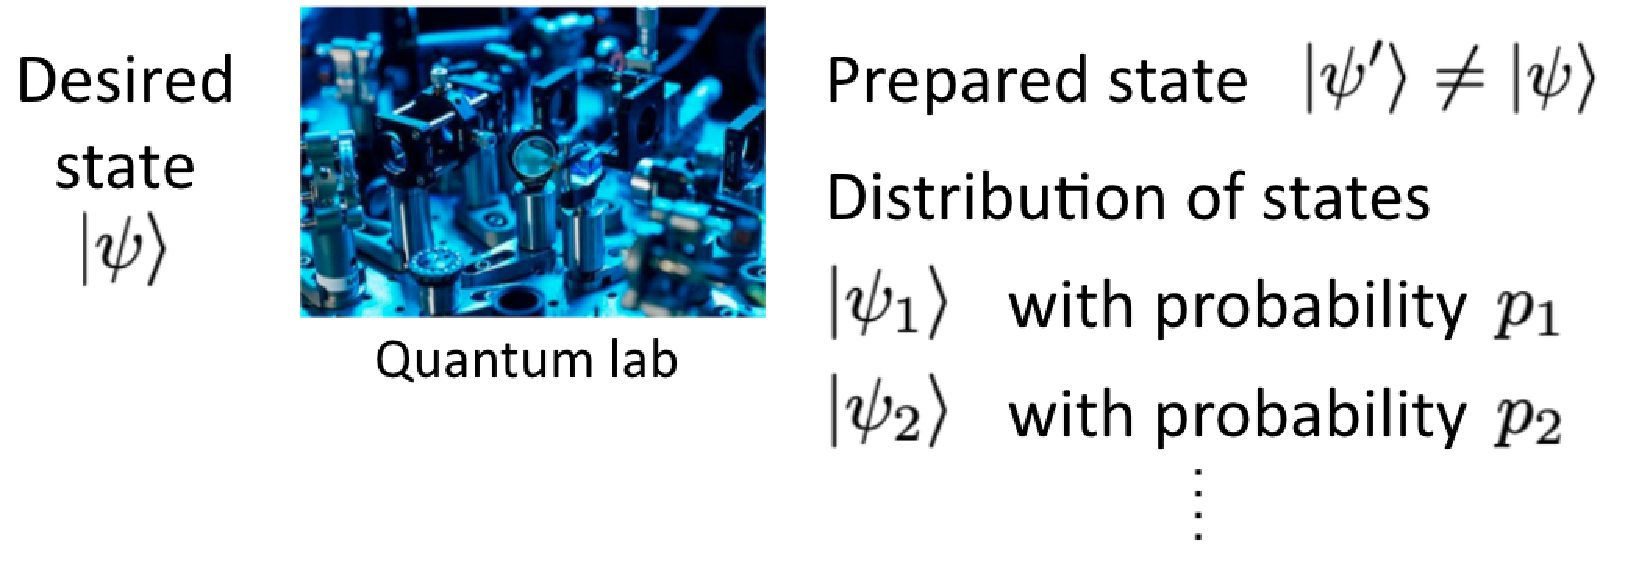
\includegraphics[width=1.0\textwidth]{lesson3/state_creation.pdf}
    \label{fig: 1}
    \begin{center}
        \caption{状態作りのノイズ}
    \end{center}
\end{figure}
例えば、 $p1$の状態で$\psi_1$の状態作ることは可能かもしれないし$p2$の確率で$\psi_2$の状態をつくったら、まあこういう分布にはなるんですがそのstate が。しょうがないんですね。これが世の中のルール、現実のことです。
それと、state、状態を作ることだけじゃなくて、stateの
\subsection{演算}
演算とかも同じなんですよね、情報処理の。その情報処理は、例えば「この$U$のユニタリー演算をかけてちょうだい」と友達に言うかもしれないんですが、出てくる結果が
$U\psi$ではない可能性は結構高い。

もうちょっと喋るとかけている$U^\prime$ (Uダッシュ)の状態が$U$ではないですね。
数学的には書くとこれも\textbf{コヒーレントのエラー}だけじゃなくて
それも\textbf{インコヒーレントのエラー}の可能性があるんですけれども、そのインコヒーレントという場合だったらこれがユニタリー演算ではないことになるかもしれない:
% processing of information
\begin{figure}[H]
    \centering
    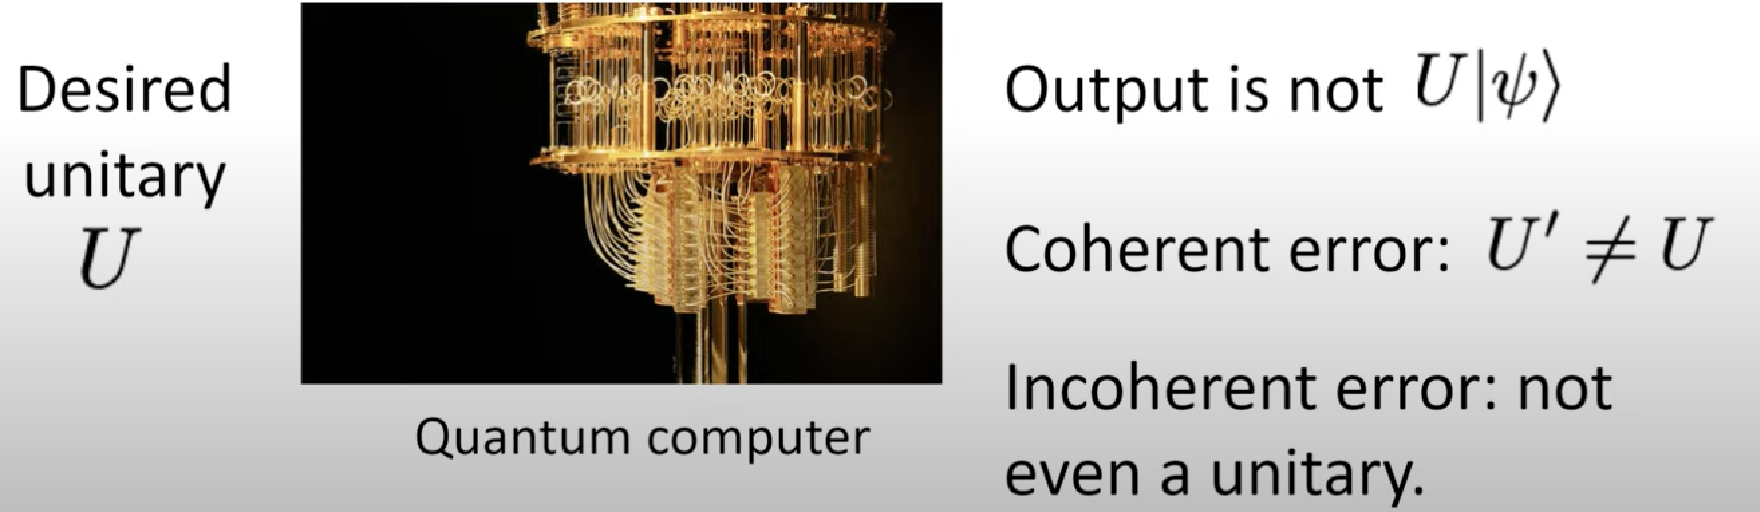
\includegraphics[width=1.0\textwidth]{lesson3/information_processisng.pdf}
    \label{fig: 1}
    \begin{center}
        \caption{演算のノイズ}
    \end{center}
\end{figure}
じゃあ、どうしましょう?
\subsection{量子通信}
Quantum Communications(量子通信)は同じですよね。
例えば、光ファイバーにstateを通すとき、まぁ最初の$\psi$のstateを送るんですが
相手に届くstateが$\psi$ではない。
% quantum communications
\begin{figure}[H]
    \centering
    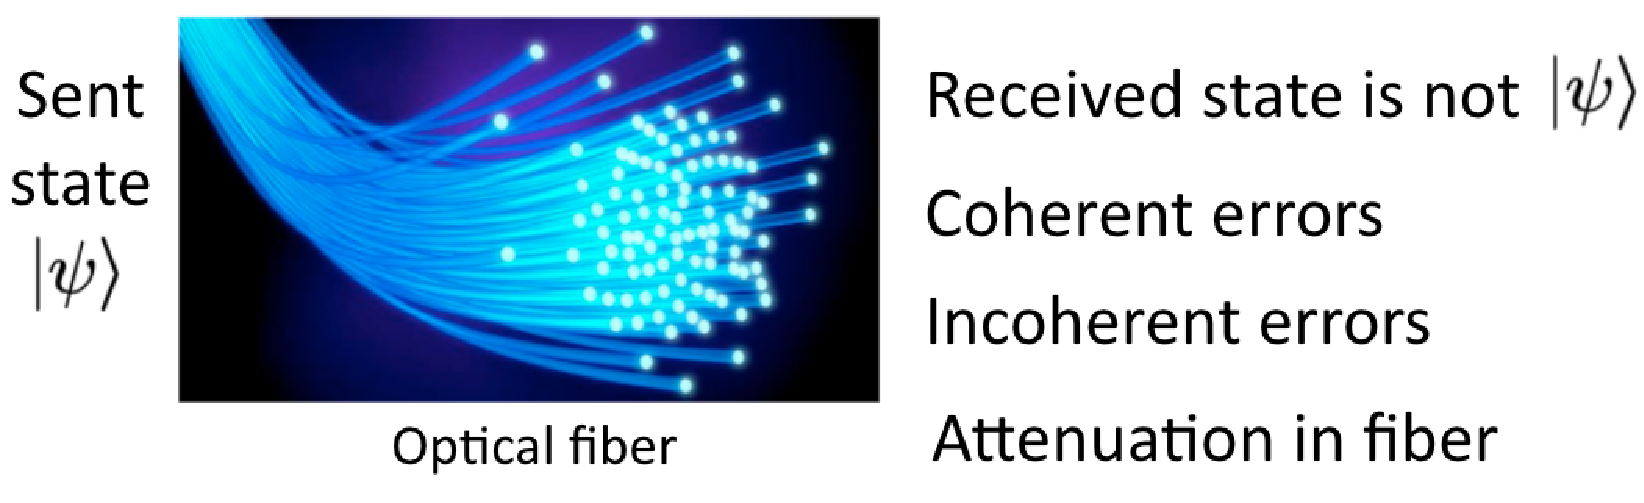
\includegraphics[width=1.0\textwidth]{lesson3/quantum_communications.pdf}
    \label{fig: 1}
    \begin{center}
        \caption{量子通信のノイズ}
    \end{center}
\end{figure}

まあそのコヒーレントエラー、つまりその先の例としてはビットフリッピ(bit flip)の$X$のユニタリー演算とか。あるいは、インコヒーレントエラーとか。あるいは光ファイバー通す光子がなくなる可能性があるでしょう。そのなくなることを\textbf{「減衰」}と言いますね。そのファイバーのattenuation(減衰)です。
\subsection{まとめ}
これが実のことなんですけれども、どうやって数学的にこれが書けるでしょう
どうやって表示して、どうやって対応できるでしょう?

\section{外積}
今までは内積を見たんですけれども、それが2つの量子状態の掛け算の一つなんですけれども。そのことは、こういうふうに書けますでしょう:
\begin{equation}
\langle a \mid b\rangle=\left(\begin{array}{ll}
a_{0}^{*} & a_{1}^{*}
\end{array}\right)\left(\begin{array}{l}
b_{0} \\
b_{1}
\end{array}\right)=a_{0}^{*} b_{0}+a_{1}^{*} b_{1}
\end{equation}
\iffalse
a のブラとbのケット(*ブラケット記法)が、

0:00:22.440,0:00:30.320
aの横のベクトルとbの縦のベクトルにすると、これがまあ

0:00:31.380,0:00:35.890
複素共役にされている

0:00:35.890,0:00:47.089
aのベクトルとbのベクトルにすると、
こういうふうになるでしょう。
\fi
\textbf{式3.1}はscalar(定数)にはなるのですが、これがComplex(複素)になるでしょう。この$a$と$b$ の順番を入れ替えると、内積が
外積になるんです。inner product(内積)がouter product(外積)になるんです。するとこういうふうに書くでしょう:
\begin{equation}
|b\rangle\langle a|=\left(\begin{array}{l}
b_{0} \\
b_{1}
\end{array}\right)\left(\begin{array}{ll}
a_{0}^{*} & a_{1}^{*}
\end{array}\right)=\left(\begin{array}{ll}
a_{0}^{*} b_{0} & a_{1}^{*} b_{0} \\
a_{0}^{*} b_{1} & a_{1}^{*} b_{1}
\end{array}\right)
\end{equation}
こうするとスカラーじゃなくて、これが行列にはなるんです。これは複素数の行列になるんです。
さて、これは何に使えるでしょう?なぜ?
外積は役に立つものです:
\begin{enumerate}
    \item 1:測定の結果に表示できます。さっきのステップで測定のことを話してたんですが、これは測定の結果、それが表示できることです
    \item 2:量子状態の新しい表示の仕方になります。それがこのレッスンの一つの大きなポイントになる。
\end{enumerate}

\subsection{測定の結果表示}
さて、$\bra{0}\ket{0}$のオペレーター、この演算と、$\bra{1}\ket{1}$のオペレーター、これの演算が、$\psi$の状態にはどう影響するのか?どう作用するのか?

じゃあ書きますと:
\begin{equation}
\begin{aligned}
|0\rangle\langle 0 \mid \psi\rangle &=|0\rangle\langle 0|(\alpha|0\rangle+\beta|1\rangle)\\
&=\alpha|0\rangle\langle 0 \mid 0\rangle+\beta|0\rangle\langle 0 \mid 1\rangle \\
&=\alpha|0\rangle
\end{aligned}
\end{equation}

$|0\rangle\langle 0 \mid \psi\rangle$これは外積かけるその$\psi$の状態なんですが、掛け算のルールによるとこの$\bra{0}$と$\psi$が\textbf{式3.3}のように内積になることも可能です。

すると、
\iffalse
この0ケット0ブラ

0:03:20.730,0:03:27.290
× $\alpha$0ケット + $\beta$1ケットが

0:03:27.290,0:03:34.710
$\alpha$ × 0 × 0ケット × 0 ブラ

0:03:34.710,0:03:42.810
× 0ケット + $\beta$ × 001にすると
\fi
$\braket{0|0}$
ゼロとゼロの内積これが正規化されているベクトルの実行の内積なんですが、その実行の内積にすると、これの結果は1です。じゃあ、それが1なりますから、$\alpha\ket{0}$を残すことになります。それから、右側にある$\braket{0|1}$、これが直交のベクトルなんですが$0$のベクトルと$1$のベクトル。直交のベクトルの内積は$1$じゃなくて、これは$0$になるんですね。そうすると、このterm(項)は消えます。
そうすると、残りの結果が$\alpha\ket{0}$になるんです。


これはこの$\ket{0}\bra{0}$のオペレーターが$\ket{0}$に\textbf{プロジェクション}することなんですが、それが射影することです。このオペレーターは$\ket{0}$の状態には射影することです。これはpauli Z basis(パウリ行列の固有状態のZ basis)の測定の結果によると、これが$+1$の結果の状態になるんです。これが
この前(レッソン2.3)の測定のことを話していたところでは、測定の結果次第では、状況が破壊することになるんですけれども。それの残りが何かの基底のベクトルになるでしょう。まあ、そういう場合には、数学的にはこういうプロジェクションのオペレーターを使うんですね。

それと、1の場合には、 $\ket{1}\bra{1}\psi$だったら、
同じルールを使うと、残りのことろは、$\beta\ket{1}$になります:
\begin{equation}
\begin{aligned}
|1\rangle\langle 1 \mid \psi\rangle &=|1\rangle\langle 1|(\alpha|0\rangle+\beta|1\rangle)\\
&=\alpha|1\rangle\langle 1 \mid 0\rangle+\beta|1\rangle\langle 1 \mid 1\rangle \\
&=\beta|1\rangle
\end{aligned}
\end{equation}
これは、$\ket{1}\bra{1}$のオペーレーターが$\ket{1}$にはプロジェクションする。射影することです。
これはPauli Z matrix、Pauli Z basis、パウリZ規定の測定の-1の結果になればいいです。

さて、\textit{他の基底で測定するとどうなるでしょう}?
さっきの話は、Pauli Z basis、つまり計算の規定なんですけれども、\textbf{Pauli X basis}、これはプラスとマイナスのbasisにもなるんですが。
すると$\ket{+}\bra{+}$の外積かける$\psi$が、そのアウトプット、その結果が測定の結果が$+1$の場合。$-1$の場合も\textbf{式1.5}で表されています:
\begin{equation}
\begin{aligned}
&|+\rangle\langle+\mid \psi\rangle=\frac{\alpha+\beta}{\sqrt{2}}|+\rangle \\
&|-\rangle\langle-\mid \psi\rangle=\frac{\alpha-\beta}{\sqrt{2}}|-\rangle
\end{aligned}
\end{equation}
これは、測定の結果が +1 の場合なんですが
\iffalse
結果が -1 の場合だったら、
$\alpha$ + 1 じゃなくて(* 訂正 "$\alpha$ + $\beta$")、$\alpha$ - $\beta$(正しくは) 
\fi
$\alpha+\beta$ じゃなくて、$\frac{\alpha-\beta}{\sqrt{2}}\ket{-}$の状態です。すると、これが -1の測定の結果にすると、これがマイナスのstateのプロジェクションにしました。

\textbf{Pauli Y basis}で測定すると:
\begin{equation}
\begin{gathered}
|i\rangle\langle i \mid \psi\rangle=\frac{\alpha-i \beta}{\sqrt{2}}|i\rangle \\
|-i\rangle\langle-i \mid \psi\rangle=\frac{\alpha+i \beta}{\sqrt{2}}|-i\rangle
\end{gathered}
\end{equation}
同じようには、$\ket{i}\bra{i}\psi$ の場合だったら$+1$の結果の場合。
$-1$の結果の場合だったら\textbf{式3.6}のように表します。


\begin{equation}
\Pi_{\pm}^{B}=\left|b_{\pm}\right\rangle\left\langle b_{\pm}\right|
\end{equation}
\textbf{式1.7}はもう一つ書けることなんですけれども、これはよく使うことがあると思います。例えば測定のbasisが大文字のΠ(パイ)の字を使えますし
\textbf{式1.7}の右側は$b$の外積にします。すると、この$\Pi$の上付き、これが基底です。これは大文字のBの基底で測定すると表示してます。
下付きのプラスマイナス、これがアウトカム。これが結果と表示します。そうすると、\textbf{式1.7}の右側は$\ket{b_+}\bra{b_+}$結果と$\ket{b_-}\bra{b_-}$の結果と表示することができます。
例とすると:
\begin{figure}[H]
    \centering
    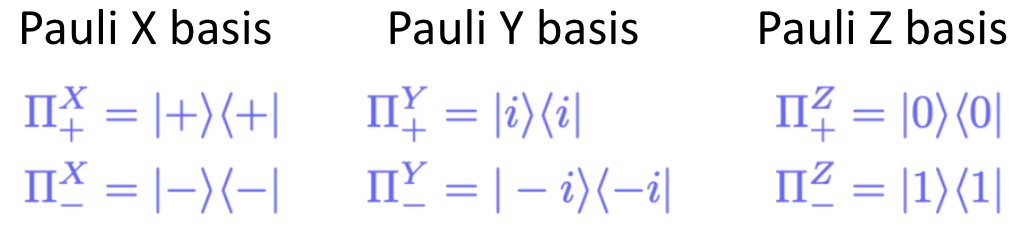
\includegraphics[width=1.0\textwidth]{lesson3/outer_product_examples.png}
    \label{fig: 1}
    \begin{center}
        \caption{$\Pi$表現の例}
    \end{center}
\end{figure}
\iffalse
Pauli Xの規定にすると、Π(パイ)の

0:08:47.420,0:08:53.779
X乗と、subプラスのところ、それが

0:08:53.779,0:09:01.220
プラスプラスの外積。
Π(パイ)をXとマイナスでは、こういうふうに書きますと、

0:09:01.220,0:09:09.300
これがマイナスマイナスの外積になります。
PauliのY basisだったら、こういうふうには書いてて、まぁこれも同様

0:09:09.300,0:09:15.840
に ii の外積と -i -iの外積になるんです。

0:09:15.840,0:09:24.819
Z basisだったら、さっきの例によると、00の外積と、11の外積になる。
\fi
\subsection{量子状態の表示}
0:09:24.819,0:09:32.920
さて、今まで話してきたことは、量子状態がケット(ket)のことを話ししていたのですが定義にすると、0のケットはこの縦のベクトル 。この$\left(\begin{array}{l}
1 \\
0
\end{array}\right)$のベクトル。

0:09:40.180,0:09:46.930
1の状態は縦のベクトルの$\left(\begin{array}{l}
0 \\
1
\end{array}\right)$。

0:09:46.930,0:09:55.830
1キュービットの状態を表示すると、
この$\psi$の変数が、この$\ket{\psi} = \left(\begin{array}{l}
\alpha \\
\beta
\end{array}\right)$の縦のベクトルなんですがこれはケットとベクトルなんですが、これも量子状態も外積に表示できるということです。

例えば、0の状態だったら$\ket{0}$と$\bra{0}$の外積を使って、
行列が$\ket{0}\bra{0}=\left(\begin{array}{ll}
1 & 0 \\
0 & 0
\end{array}\right)$ になる。
1の状態だったら、それの外積は:
\begin{equation}
    \ket{1}\bra{1}=\left(\begin{array}{ll}
0 & 0 \\
0 & 1
\end{array}\right) 
\end{equation}
になる。
もうちょっと汎用なステートにすると、この$\psi$状態にすると:
\begin{equation}
    \ket{\psi}\bra{\psi}=\left(\begin{array}{ll}
|\alpha|^2 & \alpha\beta^{\star} \\
\alpha^{\star}\beta & |\beta|^2
\end{array}\right) 
\end{equation}
\iffalse
$\psi$と$\psi$の外積にすると、$\alpha$の絶対値の自乗、

0:10:38.180,0:10:43.310
$\alpha$$\beta$* 、$\alpha$*$\beta$と

0:10:43.310,0:10:56.150
$\beta$の絶対値の自乗になることです。
\fi
多分、よく見ると、この$|\alpha|^2$と、$|\beta|^2$を見たことがあるでしょう?それの関連は後でもう少し説明します。


\section{密度行列}
今までは、Lesson 2のところには、
量子状態がkets (ケット)で表示してたんですけれども、ketsもベクトルなんですね。

例えば、そのインプットの状態は、$\psi$のketsで書きますし、それも

実の世界では、それがノイズをかけられているチャネルには、転送しますけれども出てくる結果は、$\psi$の状態ではないかもしれないんですけれども、
ここの状態にはなる、確率的に:
% noisy channel pic
\begin{figure}[H]
    \centering
    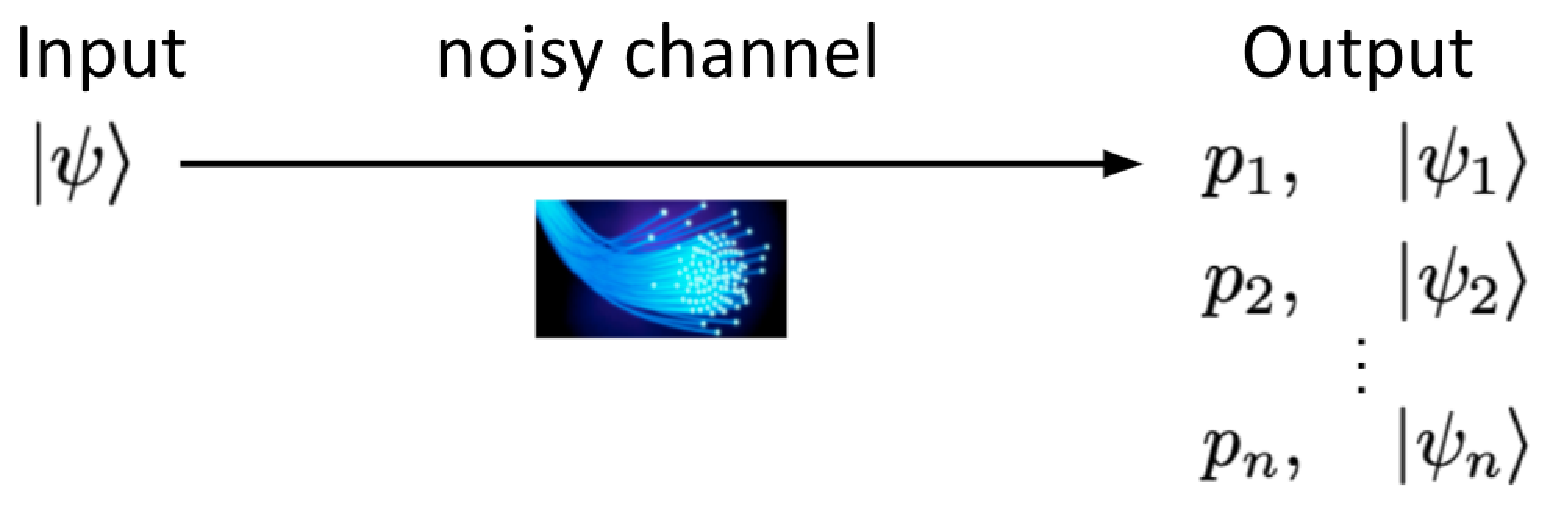
\includegraphics[width=1.0\textwidth]{lesson3/noisy_channel.pdf}
    \label{fig: 1}
    \begin{center}
        \caption{noisy channel}
    \end{center}
\end{figure}
結果としてです。例えば、$\psi_1$の出てくる確率は$p_1$で$\psi_2$が出てくる確率は$p_2$とか、
$\psi_n$の出てくる確率は$p_n$とか。
これは実世界の結果なんですけれども、これも表示できるようにしたい。
\textit{どうやってそれが表現、表示できるんでしょう}?

重ね合わせについては、普通の重ね合わせは今までは結構しゃべってるんですが、こういうstateが重ね合わせの表示の仕方にも、それを使って出来るんでしょうか?いや、できないんですね。じゃあ、なぜかちょっと見てみましょう。
その重ね合わせは、波の重ね合わせと一緒なんですけれども、その状態が完璧になっているんですね。これが、その完璧の状態は、その重ね合わせには、$0$になる確率と$1$になる確率は別になっているかもしれないんですけれど、あるいはそれは決まってないかもしれないんですが、それがstateについての知識を分かっているのと、分かってないのとは違う。

じゃあ、どうやって証明できるでしょう?どうやって表示できるのでしょう?
確率的な結果が書けるようにならないと、ノイズの影響とかではそれが計算できないから、それがやりたい。すると、今までのこのレッスンで喋っていた外積を使う。

さて、するとさっきの$p_1$、$p_2$、$p$なんとかなんとか、$p_n$になると、
$\psi_1$、$\psi_2$、$\psi$なんとか・・・、$\psi_n$にすると、それがこういうふうに書ける表現になる:
\begin{equation}
p_{1}\left|\psi_{1}\right\rangle\left\langle\psi_{1}\left|+p_{2}\right| \psi_{2}\right\rangle\left\langle\psi_{2}\left|+\ldots+p_{n}\right| \psi_{n}\right\rangle\left\langle\psi_{n}\right|
\end{equation}
\iffalse
0:02:46.610,0:02:50.960
p1 × $\psi$1の外積

0:02:50.960,0:02:59.450
+ p2 × $\psi$2の外積
+ p3 × $\psi$3の外積

0:02:59.450,0:03:08.380
続いて、+ pn × $\psi$nの外積
のようになること。
\fi
これが、一緒なんですが、この$p_1\psi_1$、$p_2\psi_2$、$p_n\psi_n$。こういうふうにしか書けない状態だったら、これが\textbf{mixed state} (混合状態)と言います。このmixed stateはそのエラー等、確率的なこと等、そういうふうに入っているということです。こういうふう表現することは、これはmixed state (混合状態)です。

例を見てみましょう:
% flip channel
\begin{figure}[H]
    \centering
    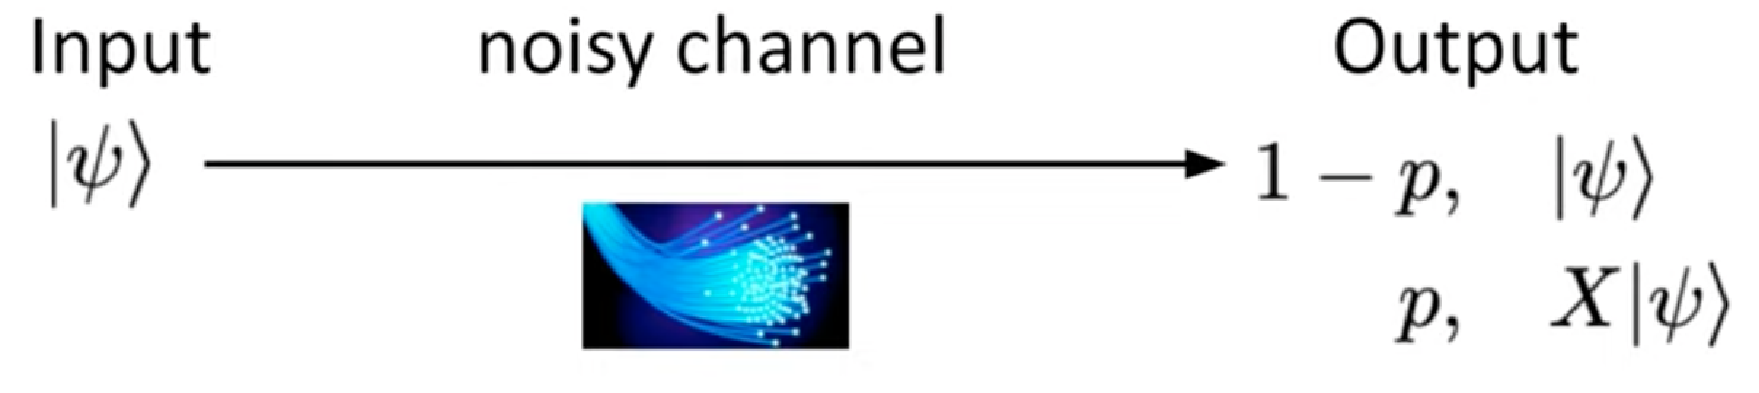
\includegraphics[width=1.0\textwidth]{lesson3/noisy_channel_bit_flip.pdf}
    \label{fig: 1}
    \begin{center}
        \caption{Noisy flip channel}
    \end{center}
\end{figure}

これはflip channelと言いますけれども、
これは古典のerror correction(エラー訂正)とかInformation theoryとか、情報理論については、これは一生の概念なんですけれども、インプットの状態が$\psi$になってまあ、noisyのchannelを通して出てくる確率は、エラーの場合の確率が、$p$の確率だったら、エラーにならない確率は$1-p$ になるでしょう。じゃあ、最初の状態が、その$\psi$の状態は、それがインプットなんですが、それがアウトプットにもしたいんですけれどもそれの確率は$1-p$。エラーになる場合には、それが$p$の確率でそのアウトプットの結果は $X\ket{\psi}$の状態です。

アウトプットには、こういうふうに密度行列を
使って、こういうふうに表現します:
\begin{equation}
\rho=(1-p)|\psi\rangle\langle\psi|+p X| \psi\rangle\langle\psi| X
\end{equation}
普通には、この密度行列の書き方にすると、変数としては、$\rho$(ロー)。
これが 、p に近い記号なんですけれども、これがギリシャ記号の$\rho$(ロー)なんですけれども。この$\rho$が\textbf{density matrix}、密度行列には使う場合が多いです。

じゃあ、\textbf{式1.11}に二つのterm(項)があるでしょう。このtermがエラーがないtermと、このtermがエラーが起こったtermですね。じゃあ、確率的には正しい状態が出てきた確率は、$1-p$で$(1-p)\ket{\psi}\bra{\psi}$の外積です。

$p$のエラーになった確率が、それが出てくる
のは\textbf{式1.11}の二項目です。
二つ目の$X$は、adjoint (随伴)しなければならないんですけれども。つまり、それは随伴行列しなければならないんですけれども、Xはself adjoint(自己随伴行列)なのでそのまま
$X$を使うことができます。

例えば、
$\ket{\psi}=0$のインプットだったら:
\begin{equation}
\rho=(1-p)|0\rangle\langle 0|+p| 1\rangle\langle 1|=\left(\begin{array}{cc}
1-p & 0 \\
0 & p
\end{array}\right)
\end{equation}
\iffalse
$\rho$(ロー)が

0:06:24.220,0:06:31.350
1- p の 0 の外積 + pの1の外積
\fi
それが$X\ket{0}$ の場合、これがbit-flip(ビットフリップ)のエラーなんですけれども、0が1になるでしょう。そうすると、計算すると、\textbf{式1 1.12}の密度行列になることです:

インプットの状態は、$\ket{\psi}=1$の状態だったら:
\begin{equation}
\rho=(1-p)|1\rangle\langle 1|+p| 0\rangle\langle 0|=\left(\begin{array}{cc}
p & 0 \\
0 & 1-p
\end{array}\right)
\end{equation}
になることです。

もうちょっと汎用的にすると、これが密度行列の事なんですけども、
これが量子状態の一番一般的な表現の仕方です:
\begin{equation}
\rho=\sum_{i} p_{i}\left|\psi_{i}\right\rangle\left\langle\psi_{i}\right|
\end{equation}

さっきのところで、ビットフリップの例もあったし、複数の出て来る可能性のことをちょっとだけ喋ってたんですけれども、もうちょっと汎用的に書くと、その$\rho$の密度行列は、\textbf{式1.14}のふうに書きます。
\iffalse
これが、sumになって、これが i のいくつかの後方のstageにあるんですが、それが 

0:07:55.629,0:07:58.520
p sub i ×

0:07:58.520,0:08:03.879
$\psi$iの外積ということになる。
\fi

これは何に使えるでしょう?
まずは、もちろん、それが今までの喋ったところは\textbf{純粋な状態}なんです。されど、pure state (純粋状態) だったら、それがこの$\rho$の表現にすると、$p_i$ はすべては0なんですが、一つだけの候補が1になっている。まあ、それがpure state (純粋状態) なんですよね。
そうすると、混合状態のmixed stateにはユニタリー演算はもうかけられている
かもしれないし、ユニタリーじゃないノイズもかけられているかもしれないし、
それだったら、この$p_i$は異なっていて、$p_i$ は1と0だけじゃなくて、いくつかの確率にはなるかもしれない。
\subsection{正規化}
レッスン2の喋ったことで、一番最初のところだったんですけれども、純粋状態は正規化しなければならない。じゃあ、それをちょっと見てみましょう。
$\ket{\psi}=\alpha\ket{0}+\beta\ket{1}$だったら、$|\alpha|^2+|\beta|^2=1$
これがその正規化状況ですね。そうすると、密度行列にはどういうふうにはなるんですかね?これは、もう一つの線形代数の概念も必要なんですけれども、これが\textbf{trace} (跡) のこと。
\begin{equation}
\operatorname{Tr}\{A\}=\sum_{i} A_{i i}
\end{equation}
\iffalse
そのtraceはdiagonal(対角)、数学的にはこういうふうに表現ができますけれども、なぜということとか、この大文字の t と小文字の r のオペレーターがこれがtraceと言いますし
\fi
Aが四角の行列をしなければならないんでするとdiagonal(対角)にある数字を足し算すると、これがtraceになる。
例えば、この 3 × 3の行列だったら:
\begin{equation}
\begin{gathered}
A=\left(\begin{array}{ccc}
A_{11} & A_{12} & A_{13} \\
A_{21} & A_{22} & A_{23} \\
A_{31} & A_{32} & A_{33}
\end{array}\right) \\
\operatorname{Tr}\{A\}=A_{11}+A_{22}+A_{33}
\end{gathered}
\end{equation}

そのNormalizationの状態、これが正規化の条件がそういうtrace使うと、そのtraceが1になるべき。例えば純粋のstateだったら:
\begin{equation}
|\psi\rangle\langle\psi|=\left(\begin{array}{l}
\alpha \\
\beta
\end{array}\right)\left(\begin{array}{ll}
\alpha^{*} & \beta^{*}
\end{array}\right)=\left(\begin{array}{ll}
|\alpha|^{2} & \alpha \beta^{*} \\
\alpha^{*} \beta & |\beta|^{2}
\end{array}\right)
\end{equation}
この$\alpha$、$\beta$の縦のベクトルと$\alpha^{\star}$、$\beta^{\star}$の横のベクトルにすると、さっきの計算した通りでdiagonal(対角)のところには、$|\alpha|^2$と$|\beta|^2$、それを合わせると:
\begin{equation}
\operatorname{Tr}\{|\psi\rangle\langle\psi|\}=|\alpha|^{2}+|\beta|^{2}=1
\end{equation}
それが先の言っていたところで、その1キュービットは、こういうふうに
すると、確率的には、何でもの$\alpha$と$\beta$振幅なんですけれども、これにすると、何かを測定すると、結果が出てくるでしょう。その結果が出てくる場合には、1になる。
\subsection{ブロッホ球表示}
さて、混合の状態も、ブロッホ球(bloch sphere)も表示できますけれども、ちょっとだけ複雑です。
さっきのpure state (純粋状態)とは違うんですね。$\psi$は純粋な状態だったら、それが球面、ブロッホ球(bloch sphere)の外側にはあるんです:
% pure state bloch
\begin{figure}[H]
    \centering
    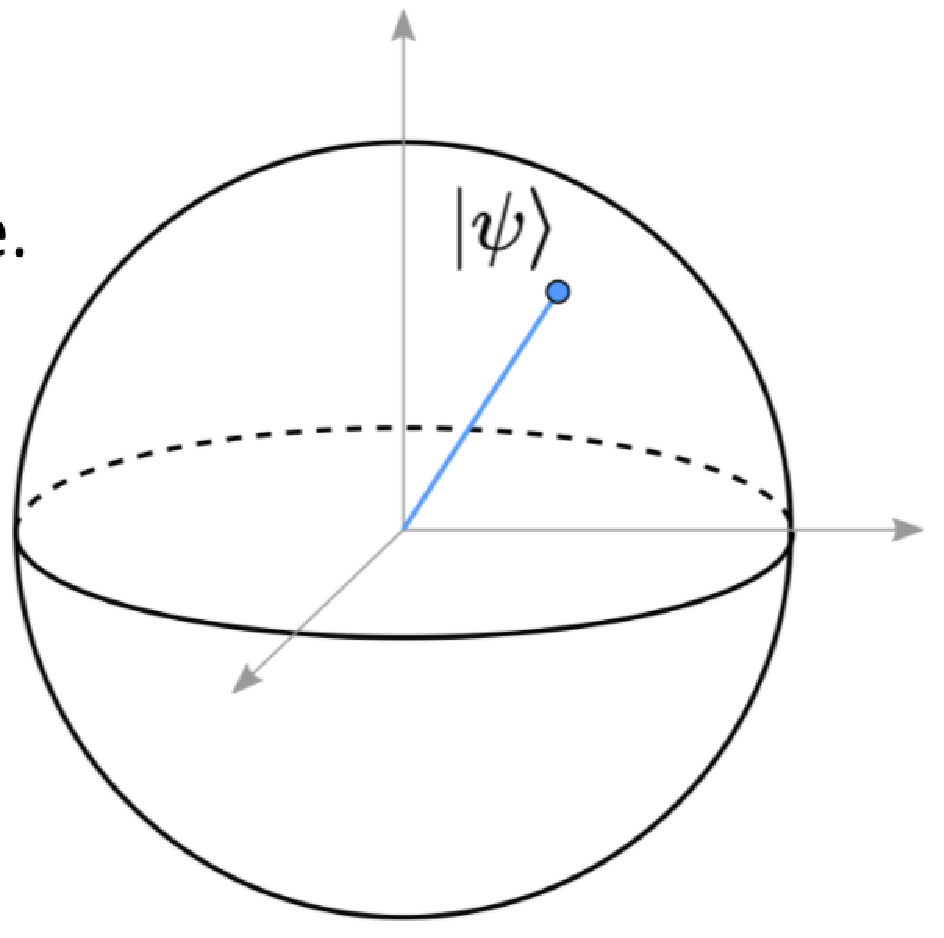
\includegraphics[width=0.5\textwidth]{lesson3/bloch_pure_state.pdf}
    \label{fig: 1}
    \begin{center}
        \caption{ブロッホ球純:純粋状態}
    \end{center}
\end{figure}
mixedの場合には、混合の状態だったら、そのベクトルの長さが、
1 じゃなくて、1より低くて、段々これがブロッホ球の中に行くことになります:
% mixed state bloch 
\begin{figure}[H]
    \centering
    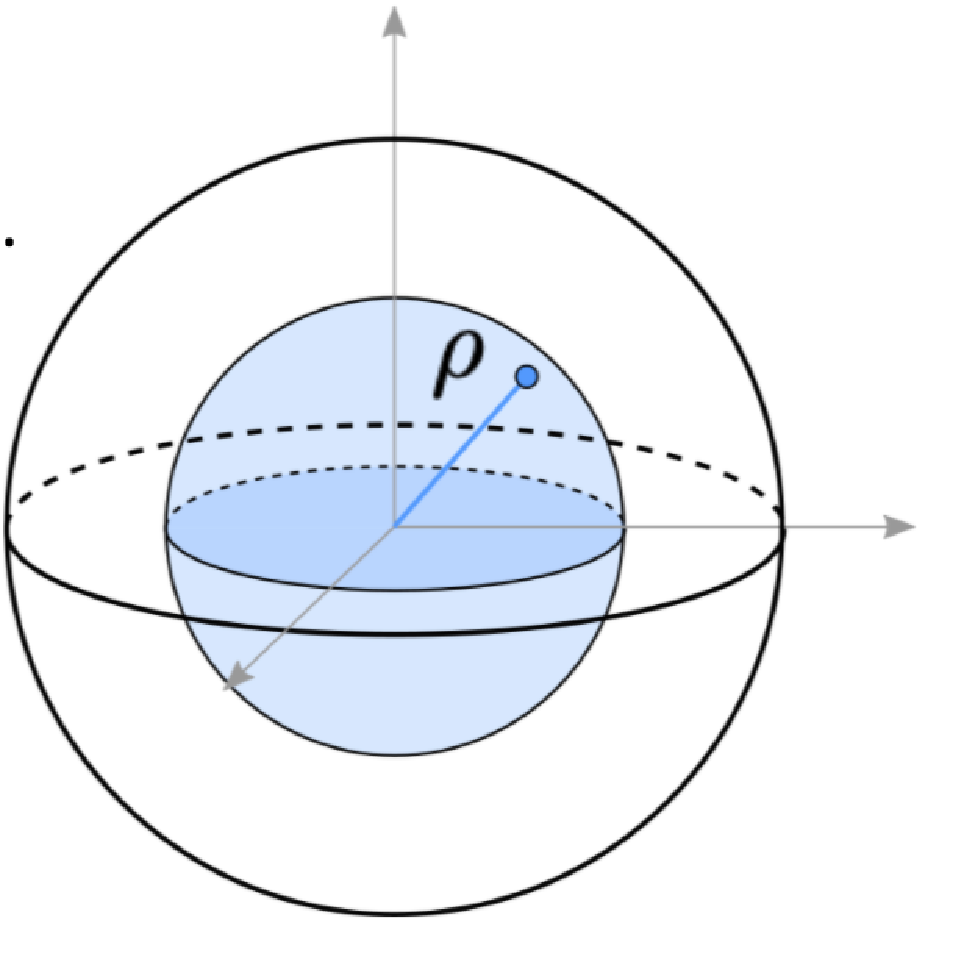
\includegraphics[width=0.5\textwidth]{lesson3/bloch_mixed_state.pdf}
    \label{fig: 1}
    \begin{center}
        \caption{ブロッホ球:混合状態}
    \end{center}
\end{figure}
そうすると、最も極端の例にすると、\textbf{maximally mixed state}と言い
ますが、それが絶対何もわかんない、それが完璧なmixed stateに何も情報が知られていないことなんですけれども、それが
ブロッホ球のど真ん中の点になるのです。
% maximally mixed state bloch
\begin{figure}[H]
    \centering
    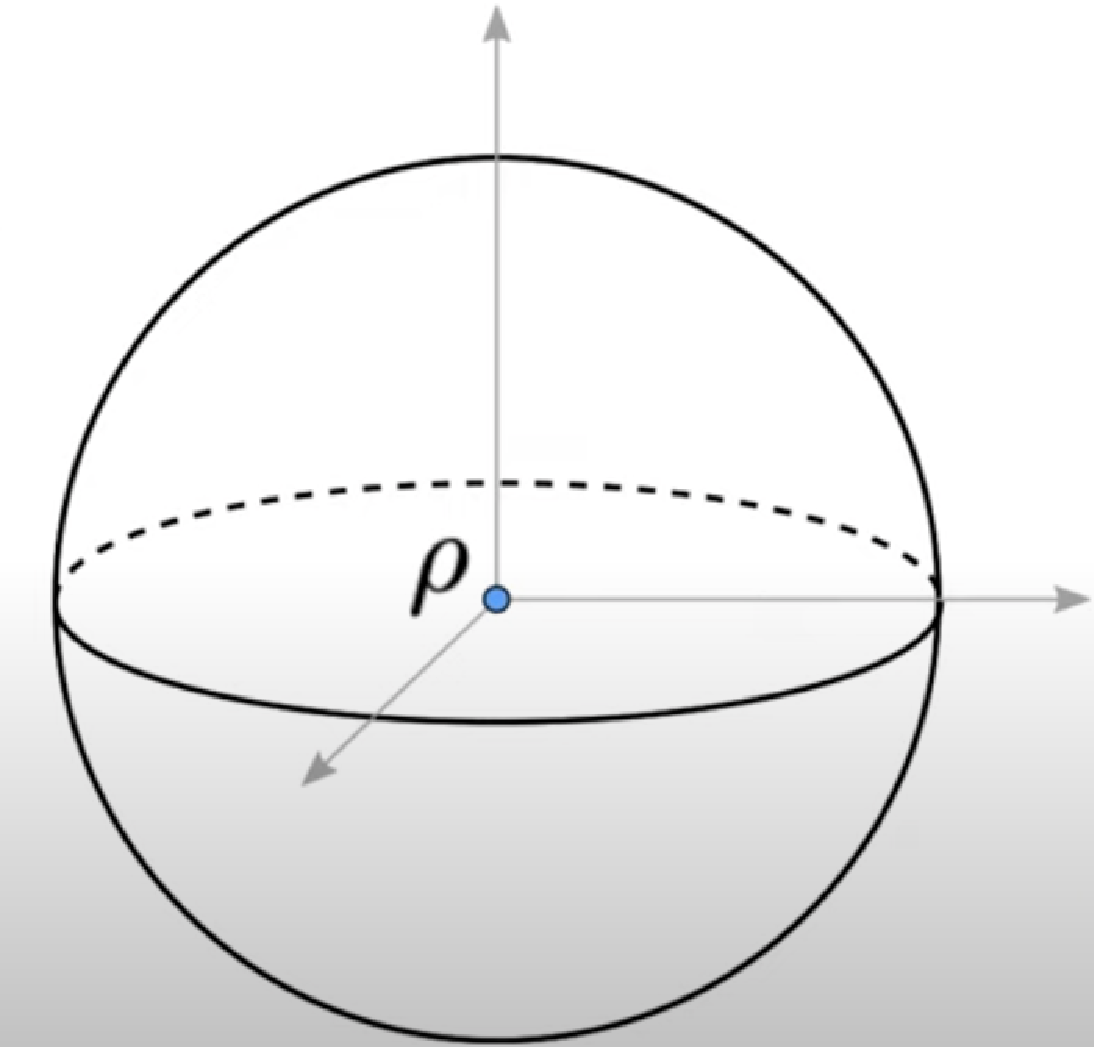
\includegraphics[width=0.5\textwidth]{lesson3/bloch_maximally_mixed_state.pdf}
    \label{fig: 1}
    \begin{center}
        \caption{ブロッホ球:最大混合状態}
    \end{center}
\end{figure}

%%%%%%%%%%%%%%%%%%%%%%%%%%%%%%%%%%%%%%
\section{純粋状態と混合状態}
一つのキュービットを考えましょう。これが、一つの例にすると重ね合わせは半分半分0と1なんですが、
それはこういうふうには書くでしょう:
\begin{equation}
|\psi\rangle=\frac{1}{\sqrt{2}}|0\rangle+\frac{1}{\sqrt{2}}|1\rangle
\end{equation}
\textbf{maximally mixed state} という状態なんですが、それが混合状態。それが何にもわからないんですが
ノイズは完璧にかけられている状況なのです。それの密度行列が、
$\rho = \ket{0}\bra{0}$の50\%と$\ket{1}\bra{1}$の50\%を表現できます。
重ね合わせ状態と混合状態を、Pauli Z basisの基底で測定しましょう:
\begin{figure}[H]
    \centering
    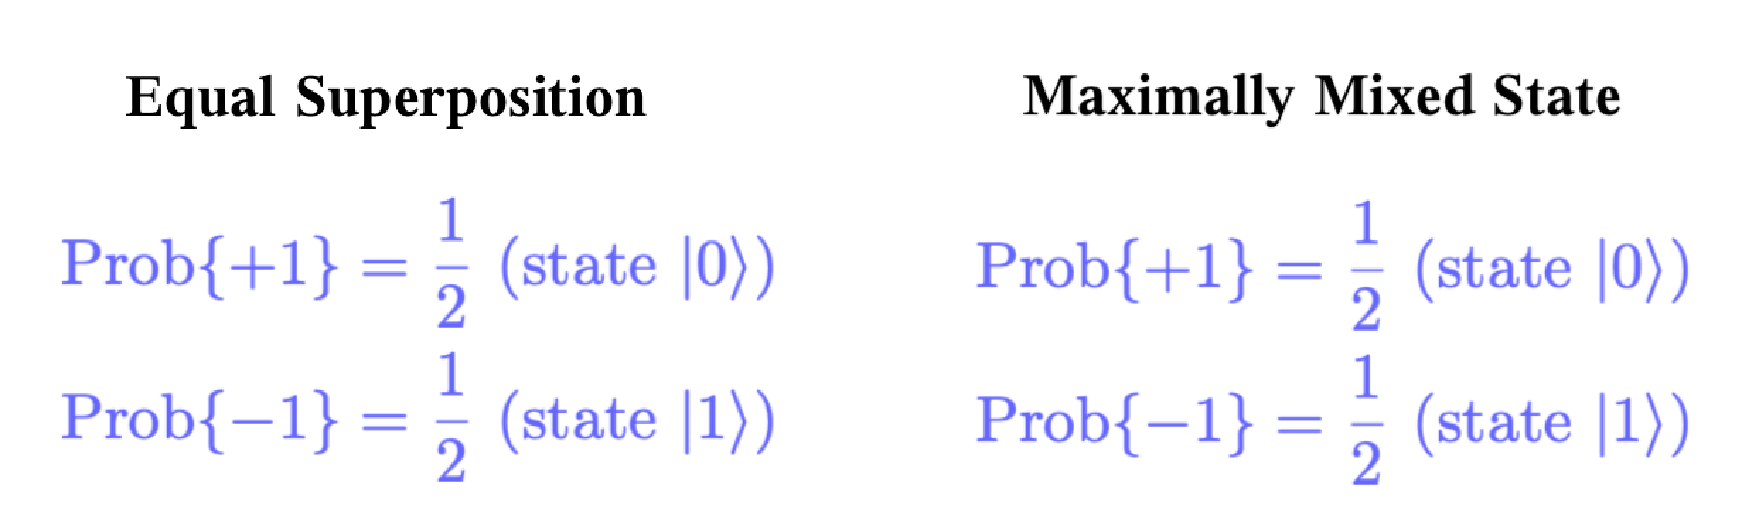
\includegraphics[width=1.0\textwidth]{lesson3/pauli_z_measurement.pdf}
    \label{fig: 1}
    \begin{center}
        \caption{Pauli Z 測定}
    \end{center}
\end{figure}
これは、計算基底と言うといいますが。すると、$+1$の確率と$-1$に出てくる確率が両方には、これが50\%の$\ket{0}$になる場合と、50\%の$\ket{1}$になる場合。Mixed stateだったら、混合状態だったら、測定すると、確率の$\ket{0}$になっている状況の確率が50\%で、$\ket{1}$になっている状態の確率、これも50\%なんですね。

じゃあ、これは同じ状態ですか?何が違うでしょう?ちょっと見てみましょう。

X basisにすると、もしかして同じか、もしかして違うんですね。見てみましょう:
\begin{figure}[H]
    \centering
    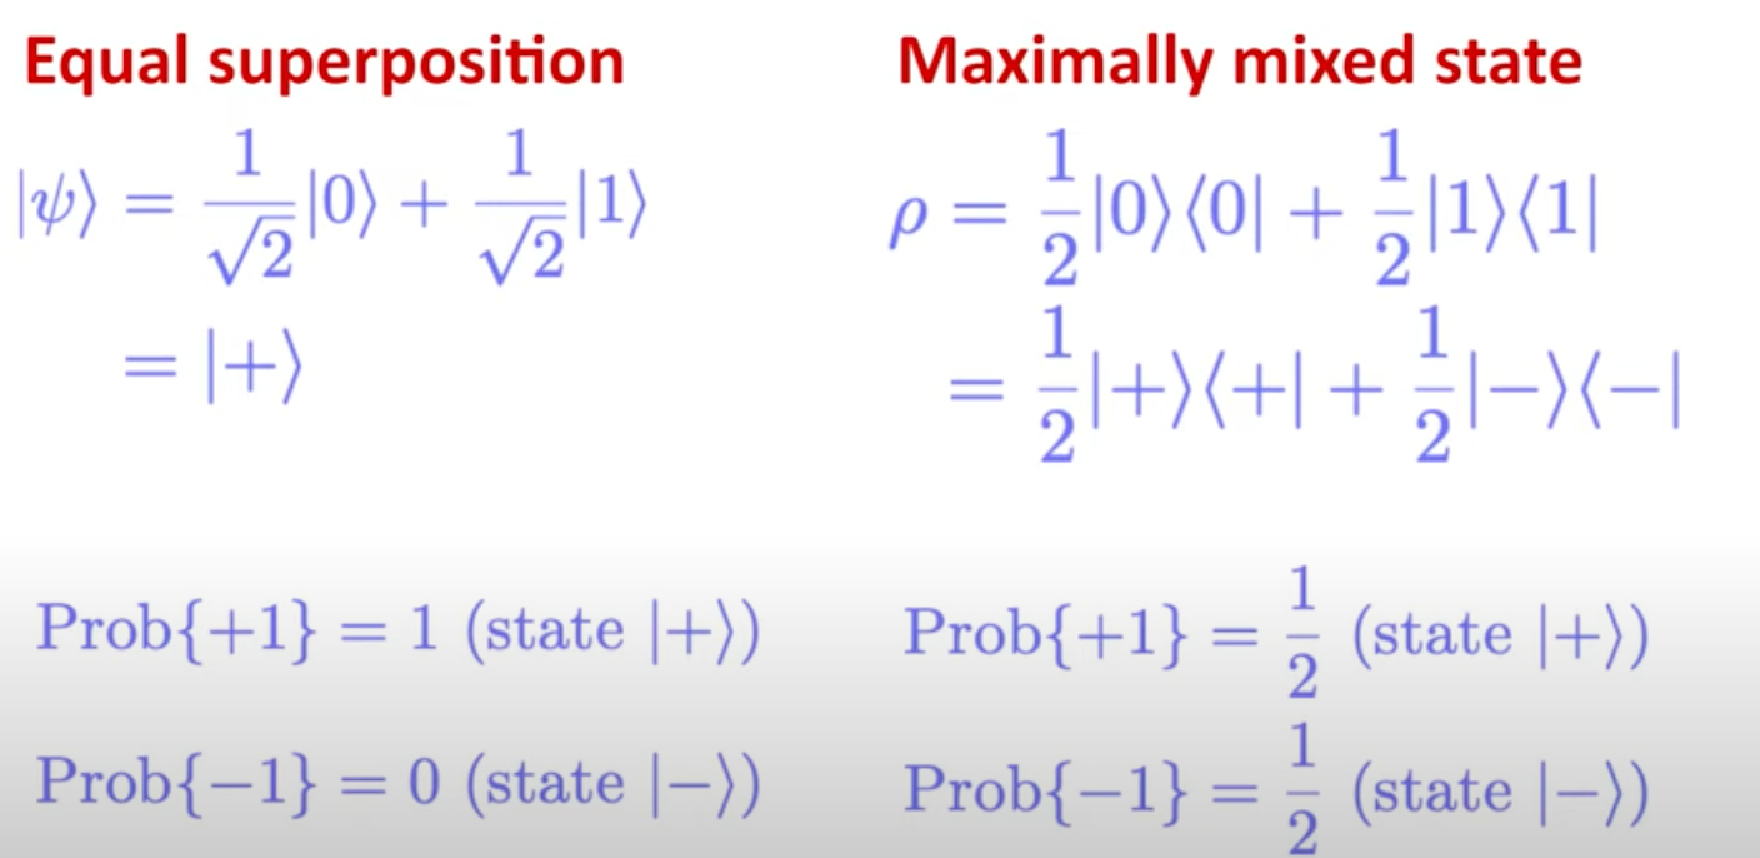
\includegraphics[width=1.0\textwidth]{lesson3/Pauli_X_measurement.pdf}
    \label{fig: 1}
    \begin{center}
        \caption{Pauli X 測定}
    \end{center}
\end{figure}

重ね合わせ状態はプラスの状態なんですが、その$\ket{+}$の状態はそれがX軸のブロッホ球の一つのてっぺんのところでしょう。だが、混合状態だったら、これがプラスの状態じゃなくて、50\%のプラスプラスの状態と、50\%のマイナスマイナスの状態。これの証明は、面白い課題にはなるかもしれません。

これを射影させることを測定してみると、$+1$の出てくる確率は
その半分半分の重ね合わせの確率が $+1$ が出てくるstateが、
それの100\%の確率です。$-1$の結果が出てくる確率はゼロです。だが、
mixed stateの場合だったら、そのプラスのstateの出てくる確率が50\%と、マイナスのstateが出てくる確率も50\%です。\textit{これは、mixed stateと重ね合わせの違いが証明できます。}
そうすると、結構使い方と、使えるところはそれの結果は結構異なる場合もありますから、是非それを注意していただきたいと思います。
\subsection{まとめ}


\begin{figure}[H]
    \centering
    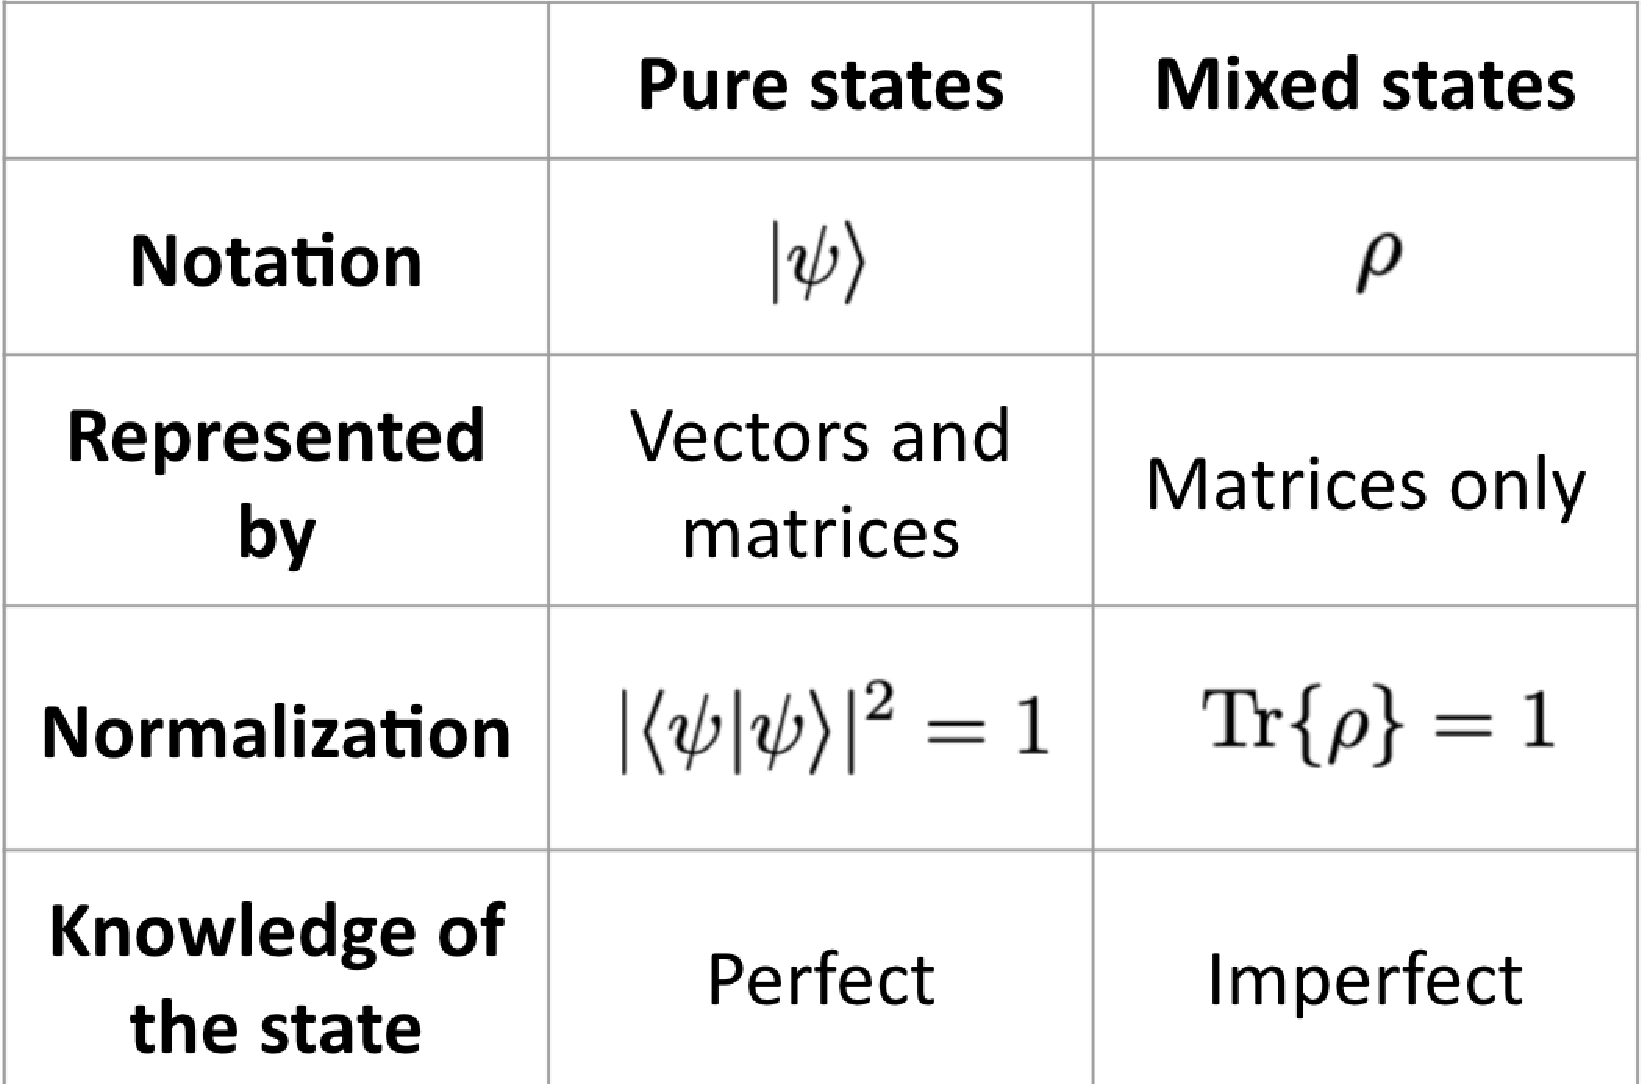
\includegraphics[width=1.0\textwidth]{lesson3/summary_table.pdf}
    \label{fig: 1}
    \begin{center}
        \caption{Pauli Z 測定}
    \end{center}
\end{figure}

サマライズすると、pure stateとmixed state、純粋のステートと混合のステート
比較してみると、Notation として、記号は何を使うのか?
\begin{enumerate}
    \item $\psi$をステートベクトルに使うんですが、mixed stateだったら、$\rho$の記号を使うでしょう。 これが密度行列になるでしょう。
    \item Pure stateだったら、ベクトルと行列の両方が可能なんですけども、mixed stateの状態だったら、密度行列だけ使えるんです。
    \item 純粋のステートだったら、正規化の条件が内積の自乗は、1に等しく なければならないんですけれども、それは自分の自己内積。密度行列だったら、その行列のtrace (跡) を1にしなければならない。
    \item どのぐらい知られているのか(分かっているのか)?純粋の状態だったら、重ね合わせになっているかもしれないんですけれども、それが重ね合わせです、とはっきり分かっているので、これがperfect (完全) な知識を持つとは言えるでしょう。ですけれども、mixed state、混合の状態だったら、それがinperfect、不完全な情報しか持ってないので、本当に作りたかった状態になっているかどうかは、何も証明ができません。
\end{enumerate}

\section{忠実度}
今まではノイズがあったpure stateは、mixed stateになることについて話をしたんですけれども、それをもうちょっと具体的に
見てみましょう:
% insert noisy channel 
\begin{figure}[H]
    \centering
    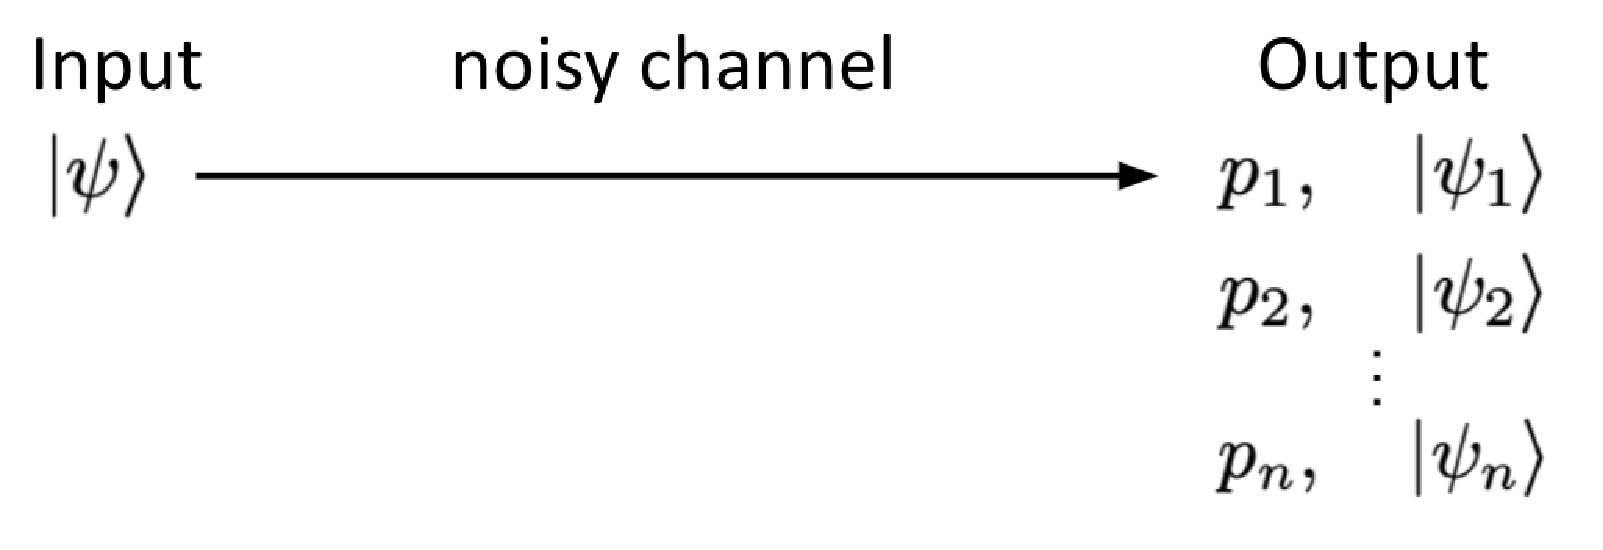
\includegraphics[width=1.0\textwidth]{lesson3/noisy_channel_buildup.pdf}
    \label{fig: 1}
    \begin{center}
        \caption{Noisy Channel}
    \end{center}
\end{figure}
例えば、上の例だったらインプットのstateは$\psi$の状況なんですが、channelを通して、それがノイズをかけられているから、確率的は他の結果が出てくる可能性がありますよね。例えば、上の例だったら、$p_1$で$\psi_1$の結果が出てくる可能性もありますし$p_2$の確率で$\psi_2$の状態が出てくる確率もあるし、段々続くと、$p_n$は低い確率で$\psi_n$の状態が出てくる可能性はありますよね。じゃあこれが複雑なんですよね。

\textit{どうやって、一つの数式だけでは、stateの状態、状況をどうやって表現、評価すればいいでしょう?}

さて、これは\textbf{Fidelity}と言います。日本語では、\textbf{忠実度}。
この忠実度の定義としては、こういうふうには計算します:
\begin{equation}
F(\rho,|\psi\rangle)=\langle\psi|\rho| \psi\rangle
\end{equation}

大文字のFで表現して、そしてそれが、2つのstateは、一つは密度行列の$\rho$と
$\psi$のステートベクトルなのですが、そうすると、こういうふうに計算します。真ん中の$\rho$を、ブラとケットではさんで、それを掛け算して結果が出てきます。その出てくる数値がFidelityです。この左側のFの大文字は、Fidelityを表示しており、この$\rho$は実のアウトプットで、この$\psi$は
作りたかった状態です。そういうふうに使います:
% Fidelity definition with annotations
\begin{figure}[H]
    \centering
    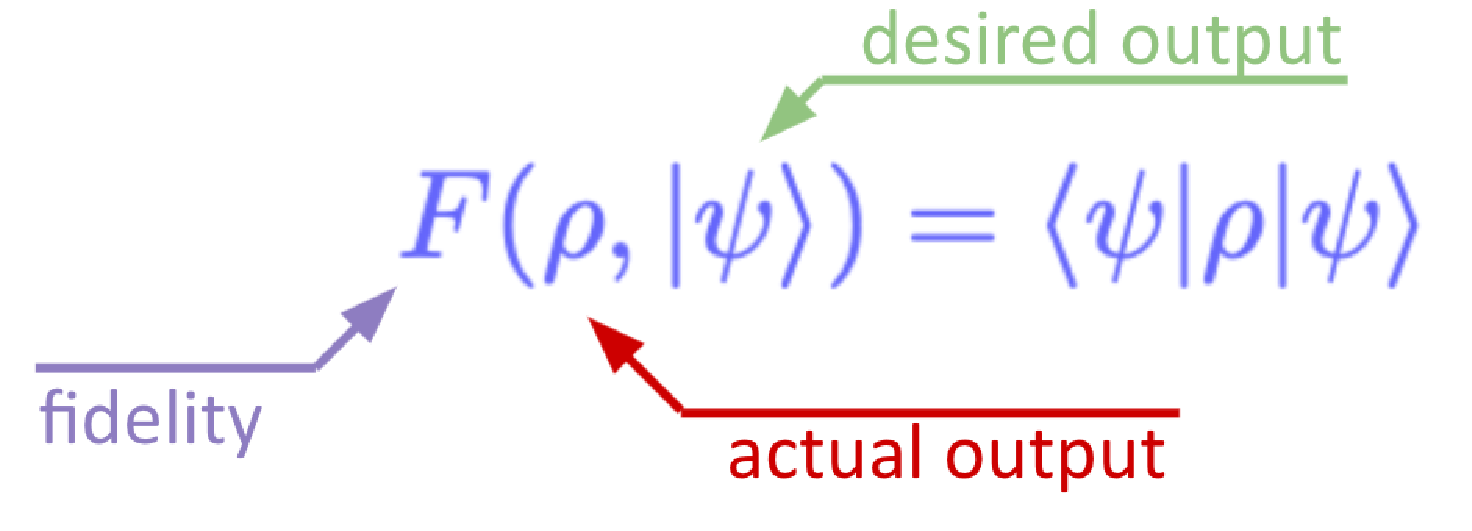
\includegraphics[width=1.0\textwidth]{lesson3/Annotated_Fidelity_defn.pdf}
    \label{fig: 1}
    \begin{center}
        \caption{忠実度の定義}
    \end{center}
\end{figure}

Fidelityは基本的にquality、品質として表示しますね。このFidelityは、0と1の間の数値なんですが、
左側の0だったら、これが欲しいstate、作りたい状態としてのorthogonal(直交)、それが直交の状態。右側の1は、それが完璧に作れたという状態です:
\begin{equation}
0 \leq F(\rho,|\psi\rangle) \leq 1
\end{equation}

\subsection{忠実度の例題}
さて、$\rho=|\psi\rangle\langle\psi$の場合だったら、$\psi$はpure stateで、それがそっちで作りたい状態だったら、本当の行列が$\rho$で出てくるので、それがケットとブラの掛け算にして、外積にして、
それがpure stateの$\rho$になります。

そうすると、じゃあどんなFidelityになるのでしょう?:

Fを計算すると、計算には細かくは一つのステップずつは書きませんけれども、
こういうふうな状態には出てきます:
\begin{equation}
\rho=|\psi\rangle\langle\psi| \quad F(\rho,|\psi\rangle)=\langle\psi \mid \psi\rangle^{2}=1
\end{equation}
そうすると、$\psi$と$\psi$の内積の自乗にはなる。
$\psi$と$\psi$の内積には、これがpure stateだったらその内積は1になるんですね。で、1の自乗は1。

もう一つの例にすると完全混合状態だったら、$
\rho= \frac{1}{2}\ket{0}\bra{0} + \frac{1}{2}\ket{1}\bra{1}$がmaximally mixed stateと言いますが、それは我々が持っている情報は何もないので、
そのキュービットの状態は、0になっている確率は50\%で、
1になっている確率も50\%で、それ以外何も情報ない。
ですけれども、その場合には、例えば、$\psi=0$を作るのを目標にしていると、じゃあどのぐらい完全混合状態はどのぐらい$\psi$に近くできたか?それを確認して、見てみましょう:
\begin{equation}
\begin{aligned}
F(\rho,|\psi\rangle) &=\langle 0|\rho| 0\rangle \\
&=\frac{1}{2}\langle 0 \mid 0\rangle^{2}+\frac{1}{2}\langle 0 \mid 1\rangle^{2} \\
&=\frac{1}{2}
\end{aligned}
\end{equation}
0と0の内積はそれが1で、0と1の内積は直交のステートなので、内積は0なので、残り数値ととして、0.5、つまりhalfになるんですね。

もう一つの例にすると、例えば、
2キュービットのステート見てみましょう:
\begin{equation}
\rho=\frac{1}{4}(|00\rangle\langle 00|+| 01\rangle\langle 01|+| 10\rangle\langle 10|+| 11\rangle\langle 11|)
\end{equation}
それの完全混合状態は、1/4の$\ket{00}$ + 1/4の$\ket{01}$ + 1/4の$\ket{10}$ + 1/4の$\ket{11}$ですね。
そうすると、例えば、作りたい状態は$\psi = \ket{00}$の場合だったら、
これもちょっと計算してみると、結果は4分の1になります:
\begin{equation}
F(\rho,|\psi\rangle)=\langle 00|\rho| 00\rangle=\frac{1}{4}
\end{equation}
$\ket{00}$と、$\ket{00}$のterm、その最初のtermは
それが1 × 1/4 なんですが、他の状態には、それが内積は0になりますから、
それも消えてしまって、残りは1/4。

Nキュービットの場合であったら、想像できるかもしれないんですけれども、
2のN乗分の1になります。
% N qubit equation
\begin{figure}[H]
    \centering
    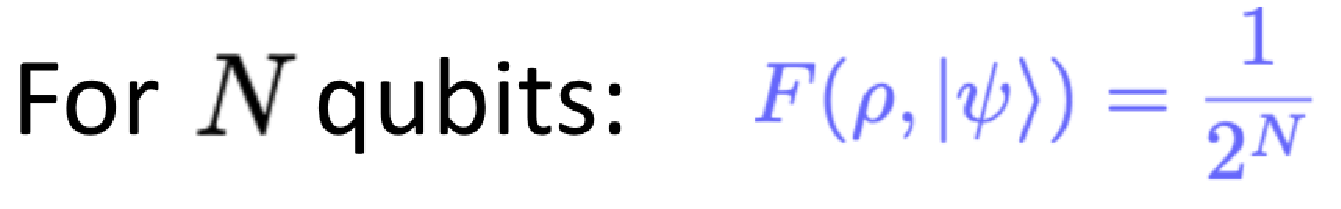
\includegraphics[width=1.0\textwidth]{lesson3/N_qubits_relation.pdf}
    \label{fig: 1}
    \begin{center}
        \caption{N-qubitsの忠実度}
    \end{center}
\end{figure}
で、1キュービットだったら、完全混合状態のFidelityは、1/2。2キュービット立ったら1/4、3キュービットだったら1/8と、それが続きます。

そうすると、例をちょっと見てみましょう。
Step 3で見たキュービットflip channelのなんですがインプットは$\psi$の状態でチャネルを通して、
アウトプットは$p$の確率でflipped(反転)されてしまう:
% noisy channel ex
% N qubit equation
\begin{figure}[H]
    \centering
    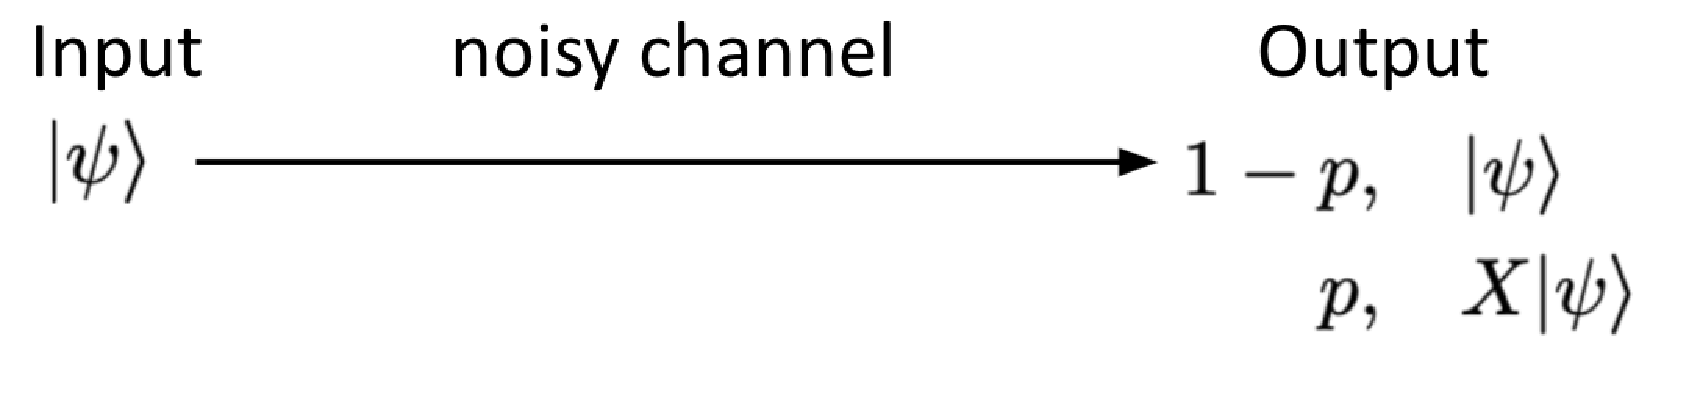
\includegraphics[width=1.0\textwidth]{lesson3/noisy_channel_ex.pdf}
    \label{fig: 1}
    \begin{center}
        \caption{Noisy channel 忠実度}
    \end{center}
\end{figure}

すると同じ、最初のインプットの状態が正しく出てくる確率は、$1-p$ になります。
じゃあこれのFidelityをちょっと計算してみましょう。
\begin{equation}
\rho=(1-p)|\psi\rangle\langle\psi|+p X| \psi\rangle\langle\psi| X
\end{equation}
まずは、$\rho$をその密度行列、Density Matrixを書いて、それが$1-p$ の$\psi$の外積+$p$ × キュービットのflippedの状態です。そのキュービットのflippedは密度行列の場合にはこのケットとブラの外積を、Xのbit-flipオペレーターで挟んで、それでを表示します。
これが完全混合状態じゃなくて、これが何かの確率的にはerrorがあったステートです。
そうすると、Fidelityを計算するとこういうふうになって結果として$Fidelity=1-p$:
\begin{equation}
\begin{aligned}
F(\rho,|0\rangle) &=\langle 0|\rho| 0\rangle \\
&=(1-p)\langle 0 \mid 0\rangle^{2}+p|\langle 0 \mid 1\rangle|^{2} \\
&=1-p
\end{aligned}
\end{equation}
つまりエラーが起こってない場合の確率になります。

\subsection{まとめ}
さて、Fidelityがあると、何の役に立つでしょう:
% Insert final summary slide 
\begin{figure}[H]
    \centering
    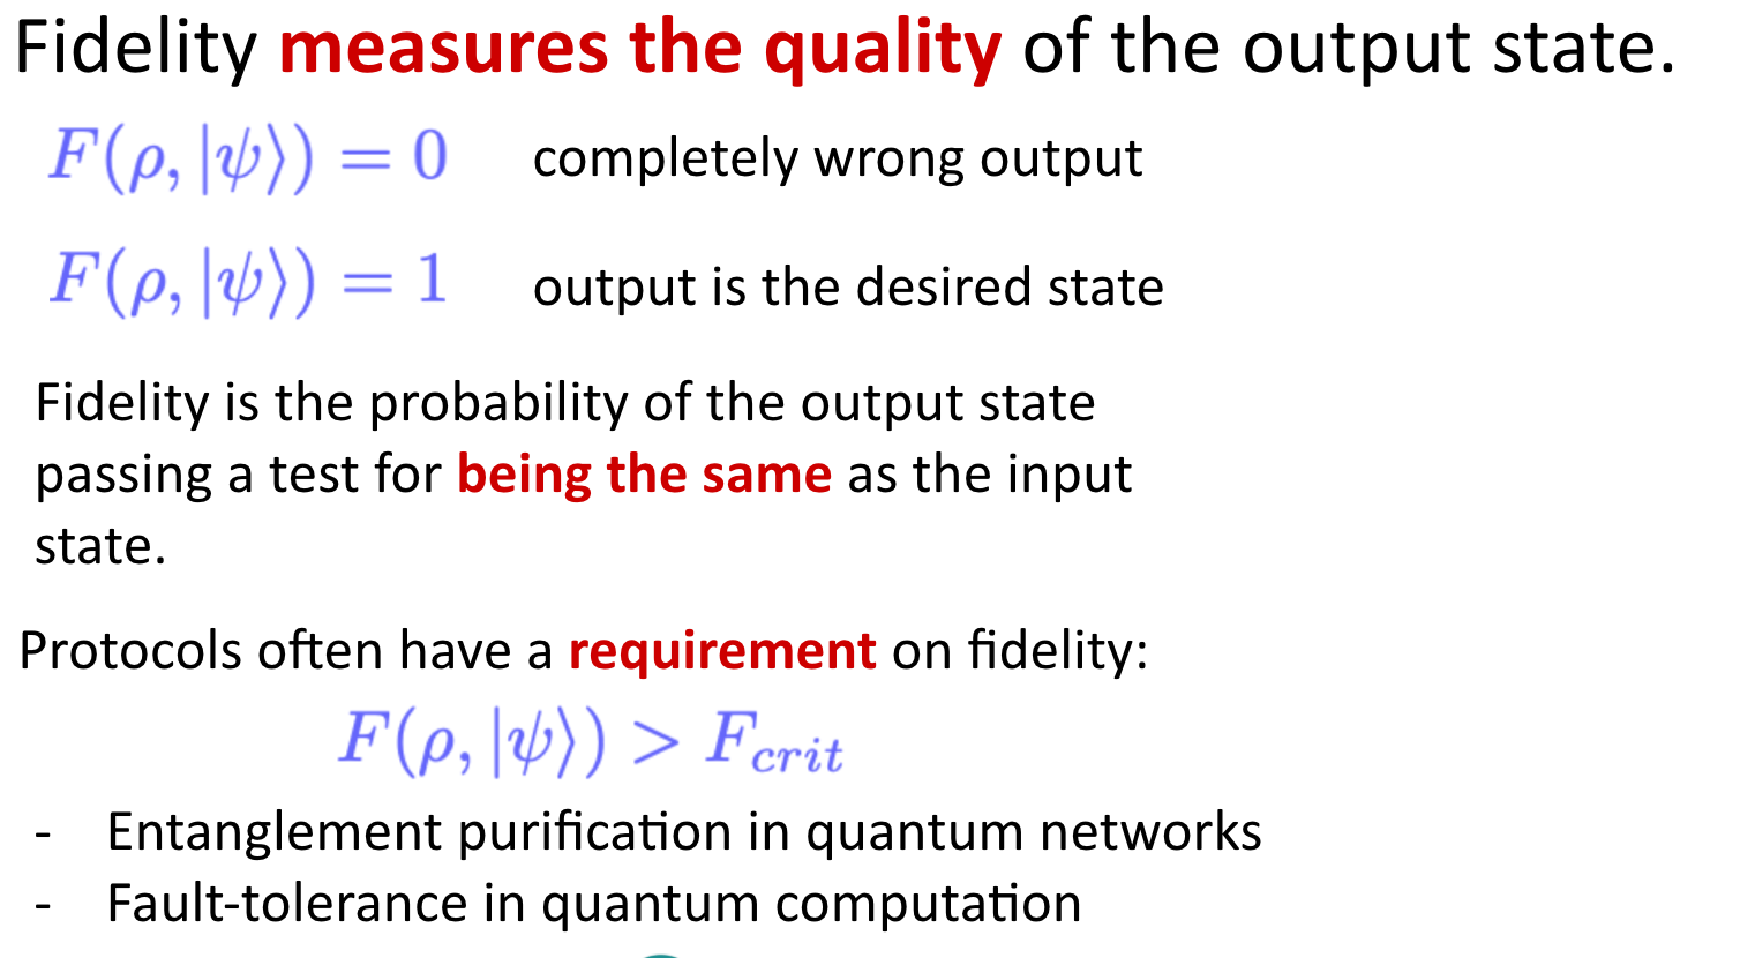
\includegraphics[width=1.0\textwidth]{lesson3/summary_fidelity.pdf}
    \label{fig: 1}
    \begin{center}
        \caption{Fidelityの魅力}
    \end{center}
\end{figure}
\begin{itemize}
  \item Fidelityというのは、忠実度であって、状態の品質を表示します。
  \item 何に使えるんでしょう?Fidelityが0だったら、これは完全に間違っている状態です。1だったら、作りたかった状態が出来ました。
  \item 基本的にFidelityは、作りたい状態ができた確率で、それはいろんな分散量子計算とか、いろんな使い方をするでしょう。この分散型のシステムによるとじゃあ、各アプリケーションが、何かのthreshold(閾値)のFidelityがあるんですけれども\textbf{Critical threshold}(臨界閾値)としては、それを超えたら、そのアプリケーションは正しく実行する可能性はあります。それ(臨界閾値)以下だったら、使えないことの状態になるんですけれども、そうするとネットワークを作っている状態の品質が足りなくて、やりたいアプリケーションは正しく実行できない可能性があります。
  \item そうすると、エンタングルメント精製、entangle purificationを使うことは可能なんですけれども。あとは、False torrentの量子計算の手法
を使えば、何とかなる可能性があります。
\end{itemize}



